\documentclass[a4paper, 11pt]{article}

% Packages
\usepackage{amsmath}
% \usepackage[toc, page]{appendix}
\usepackage{booktabs}
\usepackage{dsfont}
% \usepackage{fancyhdr}
\usepackage{graphicx}
\usepackage{hyperref}
% \usepackage{pdfpages}
\usepackage[sort&compress]{natbib}
\usepackage{subcaption}
% \usepackage[nottoc]{tocbibind}

% Location of the graphics files
\graphicspath{{figures/}}
% Set line spacing
\linespread{1.5}

\begin{document}

\title{Transfer Report}
\author{Keiran Suchak --- 200888140}
\date{\today}
\maketitle

\tableofcontents

\newpage

%\section*{Ideas}\label{sec:ideas}

%Exploring the impact of the following on the effectiveness of the filter:
%\begin{itemize}
    %\item Model non-linearity
    %\item Varying levels of data aggregation
    %\item Varying levels of observation noise
    %\item Varying frequency of assimilation
    %\item Varying level of agent knowledge (perhaps parameter estimation is
        %required here)
    %\item Varying levels of data coverage (all agents vs some agents)
%\end{itemize}

%What metrics do we use?
%\begin{itemize}
    %\item Average distance error over each agent?
    %\item Number of agents correct? What is correct?
    %\item 
%\end{itemize}

%Potential comparison with other methods:
%\begin{itemize}
    %\item Particle Filter
    %\item Unscented Kalman Filter
    %\item Probabilistic Programming
%\end{itemize}

%What do we compare?
%\begin{itemize}
    %\item Accuracy
    %\item Tractability
%\end{itemize}

\section{Introduction}\label{sec:intro}

\begin{itemize}
    \item What am I doing?
    \item Why am I doing it?
    \item How have people done it in the past?
    \item How do I plan to do it?
\end{itemize}


\section{Thesis Structure}\label{sec:structure}

%Ideas for subsequent research:
%\begin{itemize}
    %\item Further exploration of EnKF:
    %\begin{itemize}
        %\item Varying levels of data coverage:
        %\begin{itemize}
            %\item Information on all agents vs some agents
            %\item Aggregated sensor data vs individual coordinate data
            %\item Varying level of agent attribute knowledge, e.g. do we know
                %about agents' destination? If not do we attempt to fix this? If
                %yes then how?
        %\end{itemize}
        %\item How does effectiveness vary with the level of non-linearity in the
            %model?
        %\item How do we measure the level of non-linearity?
    %\end{itemize}
    %\item Comparison of EnKF with other DA methods given the same model:
    %\begin{itemize}
        %\item PF, UKF
        %\item Compare how effective they are
        %\item Compare time complexity
        %\item Compare space complexity
    %\end{itemize}
    %\item Application to a confined case study using real data:
    %\begin{itemize}
        %\item Headrow gateway pedestrian surveys
        %\item Development of city square:
        %\begin{itemize}
            %\item Planning of sensor network deployment
            %\item Use of DA both before and after developments
            %\item What would be the point here?
        %\end{itemize}
    %\end{itemize}
%\end{itemize}

This section proposes a structures for the final output of the PhD.
At present, this is expected to take the traditional form of a thesis, the
structure of which is outlined in Section \ref{sub:structure:thesis}; the
alternative option of pursuing a PhD by publication is also considered in
Section \ref{sub:structure:publication}.
The section also addresses possibilities for other research and outputs in the
form of case studies in conjunction with Leeds City Council in Section
\ref{sub:structure:case_studies}.

\subsection{PhD by Thesis}\label{sub:structure:thesis}

Given the aims and objectives outline in Section \ref{sub:intro:aims}, the
following structure is proposed for the thesis.

\paragraph{Introduction}

This section will be based on Section \ref{sec:intro}, providing the background
and rationale for the project, as well as outlining the main aims and objectives
of the investigation.


\paragraph{Literature Review}

The foundations of this section will likely mirror Section \ref{sec:lit_rev},
along with the addition of some coverage of:
\begin{itemize}
    \item The use of data assimilation schemes in conjunction with
        agent-based models in contexts other than social simulation,
    \item The use of methods other than data assimilation for real-time
        pedestrian modelling (as well as a comparison between such
        approaches and data assimilation methods),
\end{itemize}

\paragraph{Methodology}

This will be based on Section \ref{sec:method}, seeking to outline data
assimilation and how it works, and will be expanded to include any other data
assimilation schemes that I go on to use.

\paragraph{Exploring the Ensemble Kalman Filter with a simple ABM}

This section will be based upon the work presented in Section
\ref{sec:research}, expanding upon it by further exploring the impact of varying
levels of data coverage (knowledge of all agent locations vs knowledge of a
subset of agent location) and varying levels of data aggregation (knowledge of
individual agent locations vs knowledge of number of agents in a given area).
Furthermore, the research currently being undertaken in Section
\ref{sec:research} assumes that the data assimilation method has knowledge
regarding the origin and destination of each agent in the system; this is an
unrealistic assumption, and so an investigation into the impact removing such
knowledge on filter performance would also be involved. 
This part of the investigation would seek to understand how the different
factors impact the performance of the Ensemble Kalman Filter.
Furthermore, the hope is that this would act as a proof-of-concept.

\paragraph{Comparison of the Ensemble Kalman Filter with Different Models}

The research undertaken thus far has focused on implementing the Ensemble Kalman
Filter for a relatively simple agent-based model --- in many of the scenarios
for this model, agent motion is linear and deterministic.
There are likely many scenarios for which this is not the case.
This section would therefore seek to apply the Ensemble Kalman Filter to
different models of pedestrian motion with a view to understanding what facets
of pedestrian motion the method struggles to capture.

\paragraph{Comparison of Different Data Assimilation Methods}

At present, this work has focused on the use of the Ensemble Kalman Filter in
conjunction with agent-based models.
There exist, however, a number of other data assimilation methods --- some of
which are being actively applied to the same model.
This part of the investigation would seek to compare the different methods with
regards to effectiveness in improving simulation accuracy, time complexity and
space complexity.

\paragraph{Conclusion}

This section will draw together the research results, discussing them and how
they pertain to the aims and objectives and the literature review.

\subsection{PhD by Publication}\label{sub:structure:publication}

The structure outlined above pertains to the traditional format of `PhD by
Thesis'.
An alternative to this would be to pursue the `PhD by Publication' route, in
which the final submission would comprise of a series of papers along with and
introductory section and a conclusion section.
The benefits of such an approach would be that it would require that less time
was set aside at the end of the PhD dedicated solely to writing the thesis, and
ensuring that research is published and disseminated early in the career.
The risk of this approach is that it requires that the student has one paper
published, one in review and one ready to submit by the end of the PhD ---
papers should therefore be submitted well in advance to account for time taken
on corrections and alterations.
If this research were to follow such an approach, the following section may be
candidates for publication:
\begin{itemize}
    \item Exploring the Ensemble Kalman Filter with a simple ABM
    \item Comparison of the Ensemble Kalman Filter with Different Models
    \item Comparison of Different Data Assimilation Methods
\end{itemize}

The section of the methodology pertaining to the Ensemble Kalman Filter would be
covered in the first publication, with any subsequent data assimilation methods
being covered in the last publication.

%Given the work undertaken thus far (as outlined in Section \ref{sec:results}),
%there are a number of avenues along which future work may proceed.
%The first and most pressing avenue would be to further explore and develop the
%implementation of the Ensemble Kalman Filter for Agent-Based Models.
%Beyond this, in light of the parallel development of other data assimilation
%methods for agent-based models, a comparison of the Ensemble Kalman Filter with
%other methods should be pursued.
%Finally, the data assimilation scheme may be applied to a case-study scenario in
%order to show it's efficacy in working with real-world environments and data;
%such a piece of work would....
%Each of these avenues will be elaborated upon in the subsequent subsections.

%\subsection{Further Exploration of the Ensemble Kalman
%Filter}\label{sub:timetable:further}

%\subsection{Comparison with other Data Assimilation
%Methods}\label{sub:timetable:comparison}

%\subsection{Application to a Case Study}\label{sub:timetable:application}

\subsection{Case Studies}\label{sub:structure:case_studies}

Beyond the purely academic work outline so far, there is also scope to pursue
external research with Leeds City Council (who are the industrial partner for
this project).
Discussions regarding such case studies are ongoing, and may pertain to either
of the following:
\begin{itemize}
    \item \textbf{Pedestrian Motion on Briggate}: The previous work that has
        been undertaken to apply the Ensemble Kalman Filter to pedestrian
        agent-based models has focused on Briggate. 
    \item \textbf{Renovation of Leeds Station}: The renovation of Leeds Station
        is presently ongoing. There are also plans for the redevelopment of
        parts of Leeds City Square. Members of Leeds City Council are therefore
        interested in understanding the impact of such changes, and exploring
        how the different potential layouts of Leeds City Square will affect the
        flow of pedestrians.
    \item \textbf{Redevelopment of the Headrow}: The redevelopment of the
        Headrow has recently begun whereby Leeds City Council seek to remove the
        central partition in the road with a view to easing the flow of public
        transport, better providing for cyclists, and widening pedestrian
        walkways and offering more green-space.
\end{itemize}

\newpage


\section{Literature Review}\label{sec:lit_rev}

%\begin{itemize}
    %%\item Introduction to agent-based modelling
    %\item Review of methods for real-time model updating
    %\begin{itemize}
        %\item Data assimilation
        %\item Others
    %\end{itemize}
    %\item Talk about application to cellular automata too.
    %\item Whereas agent-based models focus on agents as the discrete indivisible
        %units, cellular automata focus on space as the units.
%\end{itemize}

As touched upon in Section \ref{sec:intro}, the process of developing an
agent-based model typically involves some form of model calibration.
Model calibration is the procedure of fine-tuning the model that we are using
such that it best fits the particular situation that we are seeking to model
\citep{crooks2012introduction}.
There are a large number of different manners in which we can calibrate
agent-based models \citep{thiele2014facilitating}.
These approaches typically involve making use of real-world data to estimate the
parameters and initial state of the model; this is, however, undertaken once
prior to running the model.

In some situations, we aim to simulate events in real-time (or close to
real-time).
In such situations, we are often able to observe the evolution of
the real-world system which we seek to model and consequently may wish to use
this information to recalibrate the model.
This would, however, require that we stop the simulation, undertake calibration,
and restart the model.
We therefore seek an approach that allows us to incorporate observations of the
system whilst simulating the system --- data assimilation.

As shall be seen, the application of data assimilation techniques to agent-based
models has been relatively limited --- this section seeks to review the existing
literature regarding such application.
Given the limited nature of such literature, some attention will also be given
to the application of data assimilation methods to the related modelling
technique of cellular automata.
Consequently, the section shall proceed as follows:
\begin{itemize}
    \item An introductory review of agent-based modelling
    \item A basic overview of data assimilation.
    \item A review of the attempts that have been made to implement data
        assimilation techniques to agent-based models and cellular automata.
\end{itemize}

\subsection{Agent-Based Modelling}\label{sub:lt:abm}

Agent-based models (sometimes referred to as individual-based models), have
become widely used in a range of fields including social systems (e.g.\ the
modelling of pedestrian movements \citep{liu2014agent}), systems pharmacology
(e.g.\ the evolution cellular systems and the impact of different intervention
measures \citep{cosgrove2015agent}), and ecological systems (e.g.\ the simulation
of habitat-selection in fish populations \citep{railsback2002analysis}).
Whilst there have existed a number of other other modelling techniques prior to
the introduction of agent-based models, many of them took the form of
differential equation-based models \citep{parunak1998agent}.
Such equation-based models seek to describe the behaviour of systems at an
aggregate level, often assuming some level of homogeneity in the population. 
Agent-based models, on the other hand, seek to describe the behaviour of the
individuals in the system, allowing the emergence of aggregate behaviour from
their interactions.

In agent-based models, individuals are characterised as discrete autonomous
agents in the model which can interact with each other, as well as with their
surrounding environment \citep{bonabeau2002agent}.
Such a characterisation involves the model containing information for each agent
regarding their attributes and the rules by which they evolve.
The rules pertaining to agent interaction aim to mirror the way in which we
observe interactions occurring in reality; real interactions often occur with
some level of variability and so the evaluation of the respective agent rules
often involve some level of randomness.
A model is therefore run by iterating forward through time, evaluating agent
interaction rules at each time-step.

The advantage of such an approach (and indeed other simulation approaches) when
considering the research field of pedestrian movement is that it allows for the
testing of scenarios that might not be possible in the physical setting of
reality, may be invasive or may be expensive.
Beyond this, the benefit of using agent-based modelling techniques over
equation-based methods is that they provide information to researchers regarding
behaviour at an individual level, as well as the derived aggregate system
behaviour.

The agent-based modelling approach is not, however, without its disadvantages.
One of the most obvious of these is the computational cost of running such a
model; as the scale of model increases (both in terms of the scale of the
environment and the number of agents), so do the required computational
resources \citep{bonabeau2002agent}.
Furthermore, the stochastic nature of these models typically means that they
must be run repeatedly with a given set of model parameters in order to deduce
consistent system behaviour, further increasing computational cost.
Such issues may be tackled through the use of supercomputing clusters and
parallelisation techniques.

A further disadvantage is that such a modelling technique requires a
fine-grained description of individual behaviour.
This is particularly challenging when considering human social systems which can
incorporate a range of complex competing motivations.
Failure to correctly capture the underlying agent behaviours can result in
spurious behaviours that do not match those observed in the real system
\citep{couclelis2002modeling}.

\subsubsection*{Calibration of Agent-Based Models}\label{subs:abm:calibration}

The process of calibrating an agent-based model involves identifying the values
that should be assigned to model parameters in order to achieve the expected
system behaviour.
Such parameters govern the ways in which agent interact with each other and with
their surrounding environment --- it is therefore crucial that correct values be
identified.
In some cases, it is not possible to calculate unique values for parameters, and
we instead are left with parameter sets, i.e.\ multiple combinations of
parameters that can be used to reproduce the desired behaviour; this can result
from over-paramerisation or correlation and interaction between parameters
\citep{gan2014comprehensive}.
The process of model calibration may also be further impeded by either a lack of
data or data with high uncertainty \citep{thiele2014facilitating}.

Associated with the process of model calibration is the procedure of sensitivity
analysis.
This process involves gaining an understanding of how sensitive a model is to
perturbations in parameter values \citep{kleijnen1995sensitivity}.

The remainder of this section will now go on provide a very brief overview of
some of the available calibration methods; a more exhaustive review can be found
in \cite{thiele2014facilitating}.

\paragraph{Full Factorial Design}

The most primitive method of model calibration is known as full factorial
design, whereby a comprehensive parameter search is undertaken by running the
model for every combination of parameter values \citep{thiele2014facilitating},
evaluating for each run the outputs of the model against the desired behaviour.
This method is appropriate when model runs are relatively inexpensive with
regards to compute time, and when parameters take integer values; in cases where
parameters take on non-integer values, care must be taken with regards to the
grid resolution of the parameters that are tested as this may significantly
change results.

\paragraph{Classical Sampling Methods}

Instead of the exhaustive search proposed in the form of Full Factorial Design,
Classical Sampling Methods involve sampling from the set of potential parameter
combinations.
In its most simple form, this would take the form of randomly sampling from
uniform distributions for each parameter value; however, this is ultimately very
inefficient.
Other sampling methods have therefore been developed.

\paragraph{Optimisation Methods}

Optimisation Methods are a common technique for fitting models.
They involve defining a cost function relating some aspect of model behaviour
with the corresponding aspect of the observed phenomenon; we then seek to
minimise the difference (i.e.\ the cost).
These approaches can therefore be viewed as minimisation problems over the
parameter space in which we often seek the global minimum.
Many techniques exist to achieve this goal, including simulated annealing (from
statistical physics) \citep{kirkpatrick1983optimization} and evolutionary
algorithms \citep{duboz2010application}.

\paragraph{Bayesian Methods}

Bayesian Methods seek to make use of Bayes theorem (outlined in Section
\ref{sub:lit_rev:da}) to identify appropriate parameter values
\citep{jabot2013easy}.
This is achieved by making use of our prior understanding of the statistical
distributions from which each of the parameter values are drawn; running a model
a large number of times with parameter values drawn from these distributions,
comparing our resulting model outputs with our observations with a view to
inferring the true statistical distributions of the parameters.
Due to the large number of times that models must be run, these methods can be
computationally expensive; however, with the increasing levels of computational
power available to researchers, they are gaining popularity
\citep{van2015calibration, beaumont2010approximate}.

\subsection{Data Assimilation}\label{sub:lit_rev:da}

%\begin{itemize}
    %\item Origins of filtering with Wiener filter, 1950. Only applies for
        %stationary signals.
    %\item Kalman-Bucy 1961
    %\item Stratonovich 1968
    %\item Jazwinski 1970
    %\item 
%\end{itemize}

The process of data assimilation involves making use of observations along with
prior knowledge (which, in our case, is encoded in a model) to produce
increasingly accurate estimates of variables of interest.
Such a process can be achieved through a Bayesian filtering approach
\citep{jazwinski1970mathematics, bar2004estimation}.

Under such a framework, the updating of the model state is undertaken on the
basis of Bayes Rule:
\begin{equation}
    P(A|B) = \frac{P(B|A) P(A)}{P(B)}
\end{equation}
Bayes Rule is made up of four components:
\begin{enumerate}
    \item $P \left( A \right)$: The probability of $A$, known as the
        \textbf{Prior}.
    \item $P \left( A|B \right)$: The probability of $A$ given $B$, known as the
        \textbf{Posterior}.
    \item $P \left( B|A \right)$: The probability of $B$ given $A$, known as the
        \textbf{Likelihood}.
    \item $P \left( B \right)$: The probability of $B$, known as the
        \textbf{Marginal Likelihood}.
\end{enumerate}
When applying this notation to the problem at hand, the components become:
\begin{enumerate}
    \item \textbf{Prior}, $P(\mathbf{x})$: The probability distribution
        representing the prior state of the model.
    \item \textbf{Posterior}, $P(\mathbf{x}|\mathbf{d})$: The probability
        distribution representing the updated state of the model in light of the
        observed data, that is to say the probability of the model state given
        the data.
    \item \textbf{Likelihood}, $P(\mathbf{d}|\mathbf{x})$: The probability
        distribution of the observed data given the model state.
    \item \textbf{Marginal Likelihood}, $P(\mathbf{d})$: The probability
        distribution representing the observed data.
\end{enumerate}
With the above notation, Bayes Rule becomes:
\begin{equation}
    P \left( \mathbf{x} | \mathbf{d} \right) =
       \frac{P \left( \mathbf{d} | \mathbf{x} \right)
             P \left( \mathbf{x} \right)}{P \left( \mathbf{d} \right)} 
\end{equation}
The aim of a data assimilation scheme therefore becomes to provide an update to
the  state in the form of the posterior, $P \left( \mathbf{x} | \mathbf{d}
\right)$, given new observations, $P \left( \mathbf{d} \right)$.

There exist a number of different schemes for tackling this problem which are
often divided into two groups \citep{talagrand1997assimilation}:
\begin{enumerate}
    \item \textbf{Sequential}: Upon the arrival of a new observation, the model
        state is updated at the time of the new observation; includes Kalman
        Filter (and variations thereof), Particle Filter.
    \item \textbf{Variational}: Upon the arrival of a new observation, the model
        solutions are updated at all times simultaneously; includes 3D-VAR,
        4D-VAR.
\end{enumerate}

Of the work that currently exists wherein investigators attempt to apply data
assimilation schemes to agent-based models, most make use of sequential schemes. 

\subsection[Application of Data Assimilation to Agent-Based Models]{Application of Sequential Data Assimilation to Agent-Based
Models}\label{sub:lit_rev:da_abm}

%Agent-based simulation is useful for studying people's movement in smart
%environment.
%Existing agent-based simulations are typically used as offline tools that help
%system design.
%They are not dynamically data-driven because they do not utilise any real time
%sensor data of the environment.
%In this paper, we present a method that assimilates real time sensor data into
%an agent-based simulation model.
%The goal of data assimilation is to provide inference of people's occupancy
%information in the smart environment, and thus lead to more accurate simulation
%results.
%We use particle filters to carry out the data assimilation and present some
%experiment results, and discuss how to extend this work for more advanced data
%assimilation in agent-based simulation of smart environment.

%\subsection{Rai 2013}

%Agent-based simulation is useful for studying human activity and their
%interactions in smart environments.
%Existing agent-based simulations are mostly offline tools that do not utilise
%real time information of smart environments.
%In previous work we developed a particle filter-based data assimilation method
%to assimilate real time sensor data from the environment into an agent-based
%simulation model.
%This paper extends the previous work by presenting a framework of behaviour
%pattern informed data assimilation.
%We describe the structure of this framework and focus on the task of behaviour
%pattern detection using Hidden Markov Model.
%We apply behaviour pattern detection to a smart office case study example and
%discuss how the detected behaviour pattern can inform the data assimilation in
%agent-based simulation of smart environments.

%\subsection{Wang 2015}

%Agent-based simulations are useful for studying people's movement and to help
%making decisions in situations like emergency evacuation in smart environments.
%These agent-based simulations are typically used as offline tools and do not
%assimilate real time data from the environment.
%With more and more smart buildings equipped with sensor devices, it is possible
%to utilise real time sensor data t dynamically inform the simulations to
%improve simulation results.
%In this paper, we propose a method to assimilate real time sensor data in
%agent-based simulations of smart environments based on particle filters.
%The data assimilations aims to estimate the system state, i.e. people's location
%information in real time, and use the estimated states to provide initial
%conditions for more accurate simulation/prediction of the system dynamics in the
%future.
%We develop a particle filter-based data assimilation framework and propose a new
%resampling method named as component set resampling to improve data assimilatoin
%for multiple agents.
%The proposed framework and method are demonstrated and evaluated through
%experiments using a sparsely populated smart environment.

%\subsection{Ward 2016}

%A widespread approach to investigating the dynamical behaviour of complex socia
%systems is via agent-based models.
%In this paper, we describe how such models can be dynamically calibrated using
%the ensemble kalman filter, a standard method of data assimilation.
%Our goal is twofold.
%First, we want to present the enkf in a simple setting for the benefit of abm
%practitioners who are unfamiliar with it.
%Second, we want to illustrate to data assimilation experts the value of using
%such methods in the context of abms of complex social systems and the new
%challenges these types of model present.
%We work towards these goals within the context of a simple question of practical
%value: how many people are there in Leeds (or any other major city) right now?
%We build a hierarchy of exemplar models that we use to demonstrate how to apply
%the enkf and calibrate these using open data of footfall counts in Leeds.

%\begin{itemize}
    %\item Environment:
    %\item Data source: synthetic data generated by the model.
    %\item Type of data: Sensors report presence of agent at position.
    %\item Method: Particle filter
    %\item Experiments run: different routing types, different number of
        %particles, single agent, two agents (set up such that agents are less
        %likely to interact).
    %\item Findings:
%\end{itemize}

\subsubsection{Particle Filter-based Approaches}\label{subs:lit_rev:da_abm:pf}

One of earliest pieces of work undertaken on the application of data
assimilation schemes to agent-based models of urban environments was by
\citet{wang2013data}.
In this work, they simulate a smart office environment with people in it --- a
scenario that is becoming increasingly common with the advent of the Internet of
Things \citep{zanella2014internet}.
The aim of the work was to make use of real-time data in conjunction with the
agent-based simulation to provide more accurate estimates of the occupancy of
the environment.
This was achieved using the Particle Filter method of data assimilation; the
method was chosen as it did not require the system to be Gaussian.
The particle filter method operates by holding an ensemble of realisations of
the simulation, each of which are evolved forward over time between
observations; when observations are received, the particle states are weighted
and the new state is obtained by sampling from these weighted particles.
The observations used were synthetic data generated by the agent-based model,
aiming to emulate motion sensors which would provide a binary response of
whether a person was present in a given location.

The work undertaken consisted of two experiments --- firstly simulating single
agent in the environment, then going on to simulate two agents in the same
environment.
In the case if the first experiment, the agent was simulated with two different
routing behaviours; for the first routing behaviour, the agent move forward
sequentially through a series of waypoints, whilst for the second routing
behaviour, the agent moves through a series of waypoints before turning back to
return to its initial position.
In this experiment, it was found that the simulation error decreased when the
agent was detected at each of the sensors for both routing behaviours with error
growing between detections; this is as expected --- it confirms that the
simulation becomes more accurate with the addition of further information
regarding the system.
In the case of the second routing behaviour, the simulation error also grew
following the agent's turn to head back to its origin.
In the second experiment, they aimed to simulate two agents in the same
environment, with the two agents maintaining spatial separation.
This simulation was run a number of times for different numbers of particles
with a view to establishing a relationship between the number of particles and
simulation accuracy.
It was found that as the number of particles was increased (through $400$,
$800$, $1200$ and $1600$), the simulation error decreased.
It was also found, however, that the experiments with fewer particles ($400$ and
$800$) struggled to converge, with the smaller number of particles unable to
provide sufficient coverage of the state space.
It was therefore noted that as the number of agents was increased, the method
was likely to struggle.

This final issue may be solved by an increase in the number of particles;
however, this comes with an attached increase  in the computational cost (both
in terms of compute time and space).
The implementation of the particle filter requires that a realisation of the
model be kept for each particle, resulting in growing memory requirements as
the number of particles are increased.
Furthermore, each particle is required to evolve the model for each time-step,
resulting in an increasing computational cost.

There are two subsequent pieces of research which have sought to build directly
upon the above initial investigation; each of them make use of the same
simulation model, adding different developments.

The first of these was undertaken by \citet{rai2013behavior} and aimed to add a
further layer by estimating behavioural patterns in the system.
This was achieved using a hidden Markov model which was trained on the
historical data of the system.
The investigation attempts to determine the accuracy with which the model
is able to identify the correct behaviour for agents, with accuracy being
defined as
\begin{equation}
    \frac{1}{T} \sum_{k=1}^T S_{t}^{k} - S_{t}^{real}
\end{equation}
where $T$ is taken to be the total number of simulation steps and $S$ is the
behaviour pattern state.
It is unclear, however, how this calculation is undertaken given that the
behavioural states are categories and not numerical; furthermore, the meaning
behind the state notation is note explained --- it appears that $k$ is a time-step
index, however it does not make sense to compare the behavioural state at each
time state to a static ``real'' behavioural state and the latter would likely be
a transient property.
Some indication is given that a numerical encoding of the categories has been
used for visualisation purposes, however this should not be used for arithmetic
purposes, nor should any ordinality be inferred from it.
Indeed, the results presented take the form of accuracy percentages, suggesting
that a more conventional accuracy score has been used, such as
\begin{equation}
    \frac{1}{T} \sum_{k=1}^{T} \mathds{1} \left(
                \hat{S}_k = S_{k}^{real} \right)
\end{equation}
where the indicator function, $\mathds{1} \left( \ldots \right)$, returns $1$
when the condition is fulfilled, else $0$.
The results suggest that the model developed accurately identifies the
behavioural states except for states that occur infrequently; the model performs
particularly well when identifying states in which agents are static, i.e.
\textit{outside} and \textit{in conference}.
Such supplementary information could improve the performance of data driven
simulations, likely helping the process of data assimilation for parameter
estimation.
It is worth considering, however, that the addition of this further layer to the
assimilation process would also result in a further increase in the
computational cost.

The second of the investigations to develop on the initial work by
\citet{wang2013data} was undertaken by \citet{wang2015data}, building more
directly on the original work.
This investigation made use of three different resampling schemes: standard
resampling (as used in the original investigation), component sent resampling
and mixed component set resampling.
These different schemes were applied to a series of experiments for comparison.

The first of these experiments seeks to address the use of component set
resampling.
This is achieved by testing the implementation for increasing numbers of agent
with component set resampling, and comparing against the corresponding results
when using standard resampling.
It was found that, when using standard resampling, the number of particles in
the ensemble that matched with observations decreased as the number of agents
increased; the use of mixed component resampling was found to reduce the rate at
which this occurred.
Beyond the results observed previously, this investigation also found that:
\begin{itemize}
    \item Simulation error in a single agent system increased when an agent
        turned back on itself in an area where no sensors were present.
    \item Simulation error in a single-agent system increased when an agent
        approached a 3-way intersection, offering it discretely different
        options of direction in which to travel --- the particles struggled to
        converge on the true state.
    \item Both component set resampling and mixed component set resampling
        improve on the accuracy gains provided by standard resampling for a
        multi-agent system.
    \item The improvements offered by mixed component set resampling over
        standard resampling diminish as the number of agents increases; this was
        attributed to situations when agents would crowd together, thus causing
        difficulties for particles to distinguish different agents captured by
        binary sensors.
\end{itemize}
Whilst this development appears promising, the issue of computational cost (both
with respect to space and time) remain largely unaddressed.
The investigation focuses on small agent populations ($\leq 6$), for which
ensemble sizes greater than $1000$ are typically used to ensure that the
application of data assimilation is worthwhile.
This would lead to a large increase in the cost of running such experiments. 
When modelling more realistic systems, agent populations would likely be much
larger, and consequently the number of particles required to improve accuracy
would grow.
This draws into question the tractability of such a method; it is likely that
(at least one of) either HPC or multi-threading approaches would be required in
such a situation.

\subsubsection{Kalman Filter-based Approaches}\label{subs:lit_rev:da_abm:kf}

Other investigations have sought to apply different data assimilation schemes
including the Ensemble Kalman Filter.
As shall be explained in Section \ref{sec:method}, the Ensemble Kalman Filter is an
adaptation of the original Kalman Filter \citep{evensen2003ensemble}.
This data assimilation technique was implemented in the investigation by
\citet{ward2016dynamic}, which sought to expose agent based modelling
practitioners to the technique in the context of modelling how many people are
in a major city at a given time.
This investigation consisted of two experiments.
In the first experiment, the Ensemble Kalman Filter was implemented with a
simple box model that estimated how many people were present in the box based on
probabilities of people entering and exiting.
In the second experiment, the Ensemble Kalman Filter was applied to an
epidemic-like model in which the population was split into workers and shoppers,
with works either being at home or at work, and shoppers either being
susceptible to going shopping, shopping in town or having returned home after
shopping.

The first experiment made use of synthetic data generated using the model with
randomly drawn parameter values in order to produce ground truth data.
Observations were then generated by adding normally distributed random noise to the
ground truth.
Running the filtering process with an ensemble of $100$ realisations, data
assimilation for state estimation was performed at each time-step, and it was
found that on average, the error (with respect to the synthetic ground truth) of
the model state was smaller after assimilation, as well as being smaller than
the error in the observations.
Furthermore, this approach also outperforms the theoretical steady state
calculated for the system.

Beyond this, the first experiment also aimed to carry out parameter estimation
by including the parameters, which are assumed to be unknown, in the state vector.
In doing so, estimates of the parameters are produced at both the forecasting
stage and the updating stage.
The filtering process succeeds in reducing the error in the parameters with
respect to the ground truth; despite this, the parameter estimates do not
converge on their true values, underestimating both the arrival rate and
departure rate.
The ratio of the two parameters, however, is correctly estimated, suggesting
that the data assimilation process has correctly estimated the governing
dynamics.

The second experiment aimed to model pedestrians arriving and departing at
Briggate in Leeds.
Pedestrians are divided into shoppers and workers, with each group being
governed by epidemic-like dynamics.
Shoppers are either at home before shopping (susceptible), in town shopping
(infected) or at home having returned from shopping (recovered); workers are
either at home or at work.
This approach seeks to more realistically represent pedestrian behaviour,
designating different types of people and introducing more complex behaviours
for agents deciding to enter the city.
The data used was sourced from a footfall camera on Briggate which recorded
hourly counts of the number of pedestrians arriving; as such, the primary target
of the assimilation process was the cumulative count of the number of agents to
have arrived in the city, combining both shoppers and workers.
The Ensemble Kalman Filter was applied using different ensemble sizes ($10$,
$100$ and $1000$), and it was found that as the ensemble size increased, the
accuracy of the simulation improved; it was noted, furthermore that the
improvement observed between ensemble sizes of $10$ and $100$ were much greater
than between ensemble sizes of $100$ and $1000$.
Once again, parameter estimation was undertaken; however, in this case a
particle filter-like approach was used.

Whilst this investigation displays that the Ensemble Kalman Filter can be
implemented in conjunction with an agent-based model to successfully improve the
model's prediction accuracy, it suffers from a number of shortcomings.
First and foremost, it should be noted that the models used for the
investigation are very simple in comparison to the majority of agent-based
models; indeed, the authors admit that the models used for the investigation
were not developed in the standard object-oriented framework typically used in
agent-based modelling.
The model used in the first experiment is a binary state model, with each agent
either being in the city or not in the city.
Such a model may be of use in gaining a picture of how the number of people in a
city varies over time, but does not provide any additional information with
regards to their spatial distribution within the city.

The inter-agent interaction governing their transition between the two states is
global --- this is to say that each agent's decisions are based on the state of
every other agent without considering more intricate mechanisms of attraction
and repulsion between agents \citep{helbing1995social} such as spatially local
ones.
Whilst the second experiment seeks to include a richer set of behaviours by
further segmenting the agents, it still fails to include any spatial aspect,
with agents again able to interact in a homogeneous fashion.

Beyond this, it should be noted that the inclusion of parameter estimation,
whilst not uncommon, is not a standard approach and so some attention should be
given to the impact of its inclusion in the procedure.
This may be achieved by undertaking the same investigation with and without
parameter estimation, comparing the accuracy with which the data assimilation
scheme models the state variable of interest.

%\subsection{Other Approaches}\label{sub:lit_rev:da_abm:other}

%Maritime piracy is posing a genuine threat to maritime transport.
%The main purpose of simulation is to predict behaviours of many actual systems,
%and it has been successfully applied in many fields.
%But the application of simulation in the maritime domain is still scarce.
%The rapid development of network and measurement technologies brings about
%higher accuracy and better availability of online measurements.
%This makes the simulation paradigm names as dynamic data driven simulation
%increasingly popular.
%It can assimilation the online measurements into the running simulation models
%and ensure much more accurate prediction of the complex systems under study.
%In this paper, we study how to utilise the online measurements in the agent
%based simulation of the maritime pirate activity.
%A new random finite set based data assimilation algorithm is proposed to
%overcome the limitations of the conventional vectors based data assimilation
%algorithms.
%The random finite set based general data model, measurement model, and
%simulation model are introduced to support the proposed algorithm.
%The details of the proposed algorithm are presented in the context of agent
%based simulation of maritime pirate activity.
%Two groups of experiments are used to practically prove the effectiveness and
%superiority of the proposed algorithm.

%\begin{itemize}
    %\item \cite{ward2016dynamic} --- model of pedestrians on Briggate, a 1-D
        %strip along which pedestrians walk, using enkf for both state and
        %parameter calibration.
    %\item \cite{wang2013data, wang2015data} --- agents occupying a smart
        %environment/building with a view to modelling population density, using
        %particle filter.
    %\item \cite{rai2013behavior} --- agents occupying a smart office/building,
        %using particle filter, extends \cite{wang2013data, wang2015data} by
        %incorporating a Hidden Markov Model for behaviour pattern detection.
    %\item \cite{wang2017random} --- model of maritime pirates, using random
        %finite set based data assimilation instead of kf or pf --- why? does
        %this have any relevance?
%\end{itemize}

%\subsection{Data Assimilation with Cellular Automata}\label{sub:lit_rev:da:ca}


%\begin{itemize}
    %\item WHAT ARE CELLULAR AUTOMATA
    %\item HOW DO THEY RELATE TO ABMS?
    %\item WHAT IS THE POINT OF INCLUDING THIS?
%\end{itemize}

%\begin{itemize}
    %\item \cite{li2017exploring} --- CA for urban land use, using enkf.
    %\item \cite{li2012assimilating} --- CA for urban land use, using enkf.
    %\item 
%\end{itemize}

\subsection{Cellular Automata}\label{sub:lit_rev:ca}

Much like agent-based models, cellular automata are a simulation method which
focus on prescribing behavioural rules at a microscopic scale and allowing the
emergence of macroscopic behaviour.
The two approaches differ, however, in that whilst agent-based models focus on
agents as the discrete indivisible units, cellular automata focus on space as
the units.
In such a model, the environment is divided up into a collection of spatial
cells, each of which has its own set of properties.
As the model is iterated forward through time, the cell properties are then
updated based on rules which typically rely on the properties of a cell's
neighbours.
Cellular automata are often implemented in research concerning land use, in
which it is common to discretise space.

Whilst this dissertation focuses on the application of data assimilation methods
to agent-based models, there also exists a body of literature in which
researchers make use of the same methods in conjunction with cellular automata.
Specifically considering research undertaken regarding urban land use,
investigations have been undertaken using both the Ensemble Kalman Filter
\citep{li2017exploring, zhang2011model, zhang2013urban} and the Particle Filter
\citep{verstegen2014identifying} 
This may be of interest to those concerned more broadly with the development of
real-time social simulation.

\subsection{Summary}\label{sub:lit_rev:summary}

%Drawing all of the information together.

%Issues to consider:
%\begin{itemize}
    %\item What happens when there is incomplete information? i.e. data is not
        %provided as frequently as we would like.
    %\item What happens when agent are given discrete choices that alter their
        %potential future states in a non-linear fashion?
    %\item Can better information regarding agent behaviour be used to improve
        %data assimilation?
    %\item EnKF vs PF: typically don't need as big ensemble sizes with EnKF, but
        %might not be able to handle models.
%\end{itemize}

As has been seen, there exist a small number of investigations which attempt to
implement sequential data assimilation schemes in conjunction with agent-based
pedestrian models; in each case, the filtering process lead to improvements in
the modelling accuracy.
Much of the work that has been undertaken has used the Particle Filter, and has
made use of synthetic data; the ultimate goal of developing such a technology
will inevitably be to use it with real-world data which is generated in
real-time.

Each of the two data assimilation schemes that have been used have their own
strengths and weaknesses.
The Ensemble Kalman Filter used by \citet{ward2016dynamic} are typically run
with smaller ensemble sizes, but struggle in cases when probability
distributions are non-normal. 
The Particle Filters used by \citet{wang2013data, rai2013behavior,
wang2015data} resolve this issues, offering an exact solution at the cost of
requiring larger ensemble sizes and consequently greater computation space and
time.

This work therefore seeks to build upon the work by \citet{ward2016dynamic} in
implementing an Ensemble Kalman Filter in conjunction with a agent-based
pedestrian model.

%Cellular automata can be thought of as a specific case of agent-based models in
%which the environment is characterised by a discrete grid, with the occupancy of
%each grid cell being updated over time based on the state of its neighbouring
%cells.
\newpage


\section{Method}\label{sec:method}

\begin{itemize}
    \item Kalman Filter
    \item Ensemble Kalman Filter
    \item Model
    \item Experiments
    \begin{itemize}
        \item Variation of observation noise
        \item Variation of assimilation period
        \item Variation of ensemble size
        \item Providing aggregated data
        \item Missing entrance/exit attributes and subsequent parameter
            estimation for these attributes
    \end{itemize}
\end{itemize}


\section{Undertaken Research}\label{sec:research}

Experiments:
\begin{itemize}
    \item Varying assimilation period and ensemble size, constant population
    \item Varying assimilation period and population, constant ensemble size
    \item Varying ensemble size and population, constant assimilation period
\end{itemize}

Visualisations:
\begin{itemize}
    \item Heat map of errors for ap vs es, ap vs pop, es vs pop
    \item Snapshot of model with ensemble members linked to relevant states
\end{itemize}

\subsection{Model}\label{sub:research:model}

The Ensemble Kalman Filter outlined in Section \ref{sub:method:enkf} is
implemented in conjunction with a pedestrian agent-based model known as
\texttt{StationSim}\footnote{https://github.com/Urban-Analytics/dust/blob/master/Projects/ABM\_DA/stationsim/stationsim\_model.py}
which aims to simulate pedestrians crossing from one side of the station to the
other.
StationSim has been developed under an object-oriented framework, and as such
both the model and the agent are represented by classes.
The state of each agent, $a_i$, comprises of its positions in two-dimensional continuous space:
\begin{equation}
    a_i = \left( x_i , y_i \right).
\end{equation}
The state of the model, $m$, comprises of the collection of all of the agents in the
model:
\begin{align}
    m &= \left[ a_0 , \ldots , a_N \right]^T \nonumber \\
      &= \left[ x_0 , y_0 , \ldots , x_N , y_N \right]^T,
\end{align}
where $N$ is the population size.
At each time-step, the model state is evolved by sequentially evolving the
agents.

The model is initialised by passing a number of arguments to the constructor,
including the number of agents in the population and the dimensions of the
rectangular environment.
Upon initialisation, the model generates a population of agents, each of which
are randomly allocated the following:
\begin{itemize}
    \item Entrance through which to enter the environment.
    \item Exit through which to leave the environment.
    \item Speed at which to traverse the environment.
\end{itemize}
As shown in Figure \ref{fig:sample_model_run}, entrances are located on the
left-hand side of the rectangular environment, and exits are located on the
right-hand side of the environment, with each agent seeking to traverse the
environment from their respective entrance to their respective exit.
Agents' motion across the environment is largely linear until they interact with
each other.
Where the paths of agents intersect in time and space, crowding occurs.
Faster agents attempt to pass slower agents, at times getting stuck behind them
--- this can be observed in the trails show in Figure \ref{fig:sample_model_run}
at $(x, y) \approx (65, 55)$.

The above phenomenon is a consequence of the agent behaviour outlined in Figure
\ref{fig:step}.
In Figure \ref{fig:step} (and subsequently Figure \ref{fig:act_deact}), the
\texttt{status} variable refers to whether an agent is active or not; a
\texttt{status} of 0 indicates that the agent is not active but is waiting to
become active, a \texttt{status} of 1 indicates that the agent is active and is
traversing the system, a \texttt{status} of 2 indicates that the agent has left
the system and is no longer active.
This variable controls agents' activation and deactivation behaviours outlined
in Figure \ref{fig:act_deact}.
The crowding phenomenon occurs due to the behaviour described in Figure
\ref{fig:move}, whereby agents attempt to move as far directly towards their
target destination as possible.
If they are unable to proceed forward, they engage the \texttt{wiggle} behaviour
where by they choose to move up or down (in the $y$-direction) in an attempt to
pass the obstruction in front of them; the decision to move either up or down is
made randomly with each choice carrying an equal probability.

\subsection{Experimental Setup}\label{sub:research:experiments}

With the above model in mind, a set of experiments were designed in order to
explore the way in which different factors impact the performance of the
Ensemble Kalman filter when applied to an agent-based model.
In particular, the factors that were explored were:
\begin{itemize}
    \item \textbf{Ensemble Size}: The number of copies of the model that the
        filter maintains.
    \item \textbf{Assimilation Period}: The number of time steps between each
        successive observation being used to update the model states.
    \item \textbf{Measurement Error}: The standard deviation of the noise
        applied to the ground truth data in order to obtain observations.
    \item \textbf{Population Size}: The number of agents created in the model.
\end{itemize}

In order to undertake this investigation, a class was developed in Python to
represent the Ensemble Kalman Filter.
The Python class representing the model is passed to the filter class as an
argument, along with the filter ensemble size, the frequency with which the
filter should assimilate data, and parameters governing the observational noise.
Upon construction, an instance of the filter class creates an instance of the
model, referred to as the \texttt{base\_model}, which takes the parameters given
in Table \ref{tab:model_params}.
Subsequently, an ensemble of models is created by taking deep-copies of the
\texttt{base\_model}, thus ensuring that each of the ensemble members starts
with model- and agent-attributes that match those in the \texttt{base\_model}.

The instance of the filter class steps forward through time according to the
predict-update cycle.
At each predict step, each of the ensemble member models are stepped forward
once, along with the base model; the frequency with which the filter undertakes
the update step is governed by a parameter known as the
\texttt{assimilation\_period}.
Upon reaching the update step of each cycle, the state of each of the ensemble
member models is updated according to equations found in Section
\ref{sub:method:enkf}.
The ground truth for these experiments is taken to be synthetic data generated
by the \texttt{base\_model}; observations are then generated by adding normally
distributed random noise to the ground truth at each assimilation step.

\begin{table}[h]
    \centering
    \begin{tabular}{@{}ll@{}}
        \toprule
        Variable                       & Value                         \\ \midrule
        Number of iterations           & 300                           \\
        Assimilation period            & $[2, 5, 10, 20, 50]$          \\
        Ensemble size                  & $[2, 5, 10, 20, 50]$          \\
        Observation standard deviation & $[0.5, 1.0, 1.5, 2.0, 2.5]$   \\ \bottomrule
    \end{tabular}
    \caption{Table of filter parameters for experiments.}\label{tab:filter_params}
\end{table}

\begin{table}[h]
    \centering
    \begin{tabular}{@{}ll@{}}
    \toprule
        Variable            & Value                 \\ \midrule
        Population size     & $[5, 10, 15, 20, 25$] \\
        Number of entrances & 3                     \\
        Number of exits     & 2                     \\
        Environment height  & 100                   \\
        Environment width   & 200                   \\ \bottomrule
    \end{tabular}
    \caption{Table of model parameters for experiment.}\label{tab:model_params}
\end{table}

%\subsection{Different Types of Ensemble Kalman Filter}\label{sec:method:types}

%Talk about the different types of EnKF and the implications for ensemble size
%\citep{keller2018comparing}.

%\begin{itemize}
    %\item Damping: counteract filter divergence
    %\item Localisation: reduce the effect of spurious correlations
    %\item Hybrid EnKF: Covariance matrix is made up of the weighted sum of the
        %usual covariance matrix and a separate static covariance matrix that
        %encodes prior underlying knowledge about the system
    %\item Dual EnKF: Split the state vector into state and parameters. At
        %assimilation: update parameters, recalculate forecast, update state
    %\item Normal Score EnKF: Developed to handle non-Gaussian PDFs in EnKF. At
        %assimilation: transform state, parameters and measurements into
        %Z-scores, perform EnKF update based on transformed values, transform
        %back from Z-scores
    %\item Iterative EnKF
%\end{itemize}

As outlined in Chapter \ref{sec:method}, the Ensemble Kalman Filter is a data
assimilation method which aims to approximate the effect of the original Kalman
Filter by representing the state of the model on which it is operating as an
ensemble of state samples.
The aim of applying this ensemble method is to overcome the difficulties
encountered by the original Kalman Filter when being applied to non-linear
models, and when attempting to propagate the state covariance matrix for models
with high dimensionality.
This method has been applied to an agent based model of pedestrian movement
(documented in Section \ref{sub:method:model}) with a view to reducing the error
in the model with respect to the ground truth.
This Section will therefore aim to present the results of the preliminary
experiments undertaken.
This is be achieved by first showing the impact of the filtering process on the
overall model state, then focusing in on a single agent in the model.
Finally a comparison of the model error for before updating, after updating and
the observations used to update will be provided at each of the time-steps in
which assimilation takes place.
It should be noted that this section adopts the common terminology of
``forecast'' to mean the state predicted by the model before updating, and
``analysis'' to mean the state after updating.

%\begin{figure}[h]
    %\centering
    %\includegraphics[width=\textwidth]{sample_model_run.eps}
    %\caption{Example run of StationSim for 20 agents; agents enter environment
    %through entrances on left and leave through exits on right.}
    %\label{fig:sample_model_run}
%\end{figure}

\begin{figure}[h!]
    \centering
    \includegraphics[width=0.8\textwidth]{sample_model_run.eps}
    \caption{Sample model run}\label{fig:sample_model_run}
\end{figure}

\begin{figure}[h!]
    \centering
    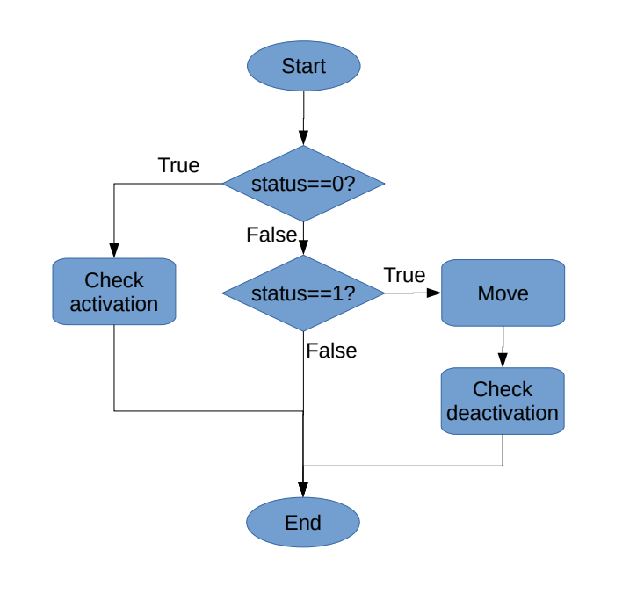
\includegraphics[width=0.8\textwidth]{step.eps}
    \caption{Flow diagram of agent step behaviour. Activation and deactivation
        behaviours are defined in Figure \ref{fig:act_deact}; movement behaviour
    is defined in Figure \ref{fig:move}}\label{fig:step}
\end{figure}

\begin{figure}[h!]
    \centering
    \begin{subfigure}[h]{0.4\textwidth}
        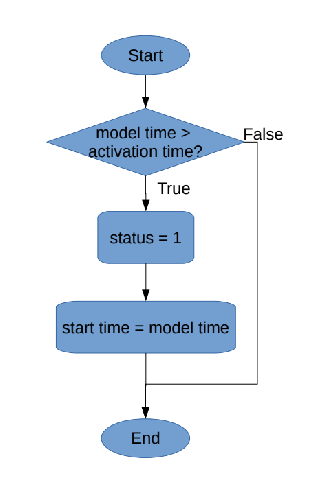
\includegraphics[width=\textwidth]{activate.eps}
        \caption{Activation}\label{fig:act_deact:act}
    \end{subfigure}
    ~
    \begin{subfigure}[h]{0.3\textwidth}
        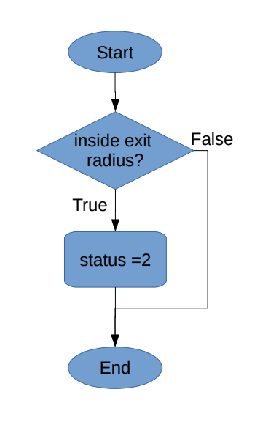
\includegraphics[width=\textwidth]{deactivate.eps}
        \caption{Deactivation}\label{fig:act_deact:deact}
    \end{subfigure}
    \caption{Flow diagrams of agent behaviours for activation and deactivation}
    \label{fig:act_deact}
\end{figure}

%\begin{figure}[h]
    %\centering
    %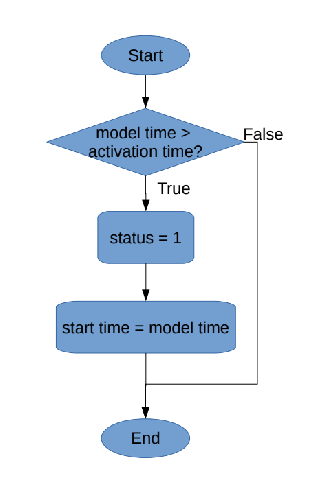
\includegraphics[width=0.5\textwidth]{activate.eps}
    %\caption{Flow diagram of agent step behaviour}
%\end{figure}

%\begin{figure}[h]
    %\centering
    %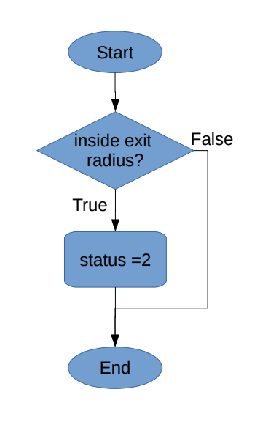
\includegraphics[width=0.5\textwidth]{deactivate.eps}
    %\caption{Flow diagram of agent step behaviour}
%\end{figure}

\begin{figure}[h!]
    \centering
    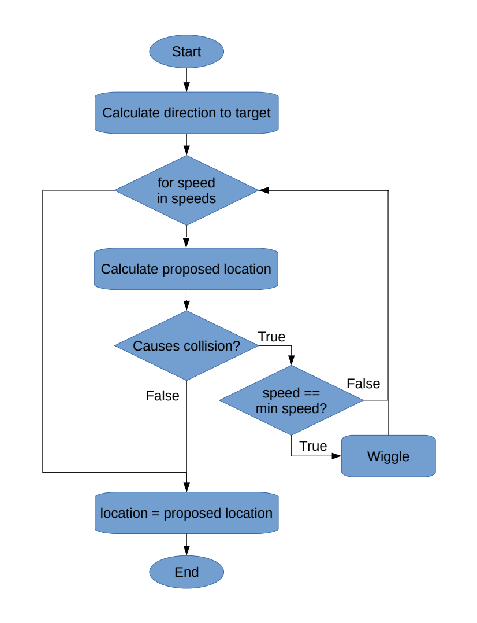
\includegraphics[width=0.8\textwidth]{move.eps}
    \caption{Flow diagram of agent movement behaviour}\label{fig:move}
\end{figure}



\section{Research Timetable}\label{sec:timetable}

\begin{itemize}
    \item Talk about thesis structure.
    \item Derive tasks from structure.
    \item Given brief overview of the task scheduling.
\end{itemize}

This section aims to outline how the remaining time in the PhD will be
allocated.
In Section \ref{sec:structure}, the structure for the PhD Thesis was proposed.
This structure lends itself to three phases of research, each pertaining to an
objective:
\begin{itemize}
    \item Objective 1: exploring the Ensemble Kalman Filter with a simple ABM.
    \item Objective 2: comparing the effectiveness of the Ensemble Kalman Filter
        when applied to different models.
    \item Objective 3: comparing the effectiveness of the Ensemble Kalman Filter
        with other data assimilation methods.
\end{itemize}
These objectives are timetabled as shown in the Gantt chart in Figure
\ref{fig:gantt_chart}.
The Gantt chart also proposes some of the conference that may be attended to
present parts of the research; GISRUK in the Spring of 2020 would provide the
opportunity to present the results of Objective 1, SIMSOC in the Autumn of 2020
would provide the opportunity to present the results of Objective 2 and SIMSOC
in the Autumn of 2021 would provide the opportunity to present the results of
Objective 3.
Subsequent RSG meetings are also expected to fall approximately around the end
of each of the Objectives.

\begin{figure}[h!]
    \centering
    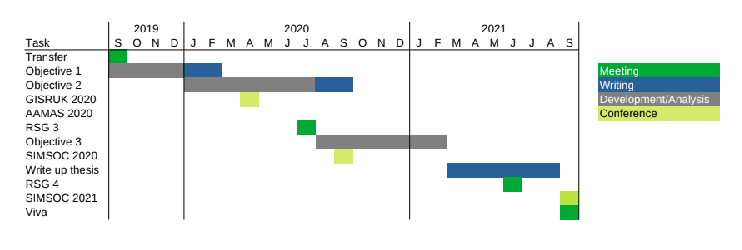
\includegraphics[width=\textwidth]{gantt_chart.eps}
    \caption{Gantt chart outline allocation of time over next two
    years.}\label{fig:gantt_chart}
\end{figure}


\section{Training Plan Review}\label{sec:training}

\subsection{Training Provided}\label{sub:training:provided}

The training provided thus far has take two form --- technical training
undertaken as taught modules on the CDT programme and non-technical training
pursued via other avenues.
Aside from the core set of modules undertaken for the CDT, I have also
undertaken the following option modules:
\begin{itemize}
    \item Big Data Consumer Analytics
    \item Parallel and Concurrent Programming (COMP5811M)
    \item Programming for Geography Information Analysis: Advanced Skills
        (GEG5790M)
\end{itemize}
These have aimed to gain a better understanding data scientific tools and to
improve my programming knowledge.
The other non-academic forms have training that I have undertaken are as
follows:
\begin{itemize}
    \item Foundations in Teaching (University of Leeds) --- Provided with an
        introduction to teaching and demonstrating as a PGR.
    \item Identifying Impact Goals (University of Leeds) --- Learned about
        reframing research with a view to achieving impact.
    \item Networking (University of Leeds) --- Gain skills for professional
        networking at conferences.
    \item Time Management (University of Leeds) --- Reviewed methods for time
        management.
    \item Literature Searching (University of Leeds) --- Learned about how to
        undertake more thorough and systematic literature reviews.
    \item Facilitator training (Turing Institute Data Study Group) --- Gained
        interpersonal skills and a greater understanding of how to manage a
        research project.
\end{itemize}

\subsection{Training Required}\label{sub:training:required}

The training provided thus far has been substantial; consequently, comparatively
little time will be spent seeking training, with more time being allocated to
PhD research.
The training that shall be sought, however, will focus on writing:
\begin{itemize}
    \item Writing for Academic Publication --- The CDT is hosting a workshop on
        getting work published at its annual event this month which I plan to
        attend.
    \item Thesis Writing --- The ODPL offers a series of workshops on developing
        writing skills specifically focused on thesis writing.
\end{itemize}


%\appendix
%\section{Code Documentation}\label{sec:cod_docs}



%\section{Derivation of Ensemble Kalman Filter}\label{sec:enkf_derivation}



\bibliographystyle{agsm}
\bibliography{references}

\end{document}
